% =============================================================================
% OpenFireWatch — Handbuch (Deutsch)
% Übersetzt für drei Lesergruppen: Einsatzkräfte, interessierte Öffentlichkeit
% und Entwickler. Übersetzung mit: latexmk -pdf handbuch.tex
% =============================================================================
\documentclass[11pt,a4paper,DIV=12,parskip=half]{scrartcl}

\usepackage[utf8]{inputenc}
\usepackage[T1]{fontenc}
\usepackage[ngerman]{babel}
\usepackage{lmodern}
% Deutsche Anführungszeichen („so"), sprachabhängig über babel gesteuert.
\usepackage[autostyle=true,german=quotes]{csquotes}
\usepackage{microtype}
\usepackage{graphicx}
\usepackage{booktabs}
\usepackage{tabularx}
\usepackage{xcolor}
\usepackage[most]{tcolorbox}
\usepackage{enumitem}
\usepackage{fancyhdr}
\usepackage[hidelinks]{hyperref}

% --- Farben aus der Anwendung ------------------------------------------------
\definecolor{ofwRot}{HTML}{C21807}
\definecolor{ofwOrange}{HTML}{C87A00}
\definecolor{ofwGrau}{HTML}{4A5568}
\definecolor{ofwHell}{HTML}{F4F5F7}

\hypersetup{colorlinks=true, linkcolor=ofwRot, urlcolor=ofwRot}

% --- Kopf- und Fußzeile ------------------------------------------------------
\pagestyle{fancy}
\fancyhf{}
\fancyhead[L]{\small\color{ofwGrau}OpenFireWatch — Handbuch}
\fancyhead[R]{\small\color{ofwGrau}\leftmark}
\fancyfoot[C]{\small\color{ofwGrau}\thepage}
\renewcommand{\headrulewidth}{0.4pt}

% --- Hinweiskästen -----------------------------------------------------------
\newtcolorbox{hinweis}[1][]{colback=ofwHell, colframe=ofwGrau,
  boxrule=0.4pt, arc=2pt, left=8pt, right=8pt, top=6pt, bottom=6pt,
  fonttitle=\bfseries, title=#1}
\newtcolorbox{warnung}[1][Wichtig]{colback=ofwRot!5, colframe=ofwRot,
  boxrule=1pt, arc=2pt, left=8pt, right=8pt, top=6pt, bottom=6pt,
  fonttitle=\bfseries, title=#1}
\newtcolorbox{fuerwen}[1][]{colback=ofwOrange!8, colframe=ofwOrange,
  boxrule=0.6pt, arc=2pt, left=8pt, right=8pt, top=5pt, bottom=5pt}

\newcommand{\zielgruppe}[1]{\begin{fuerwen}\textbf{Für wen:} #1\end{fuerwen}}

\begin{document}

% =============================================================================
\begin{titlepage}
\centering
\vspace*{2cm}
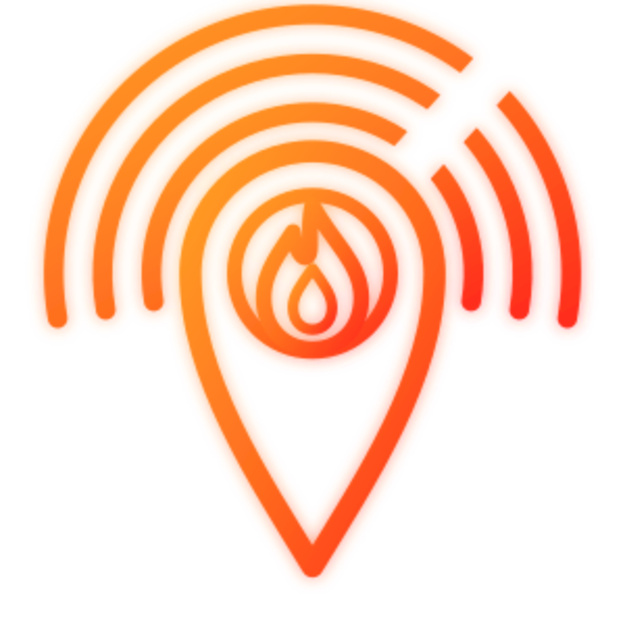
\includegraphics[width=4.5cm]{img/logo.pdf}

\vspace{1.2cm}
{\Huge\bfseries OpenFireWatch\par}
\vspace{0.4cm}
{\Large Geografisches Frühwarnsystem für thermische Anomalien\par}

\vspace{0.8cm}
{\large\color{ofwGrau} Handbuch für Einsatzkräfte, Betreiber und Entwickler\par}

\vspace{2cm}
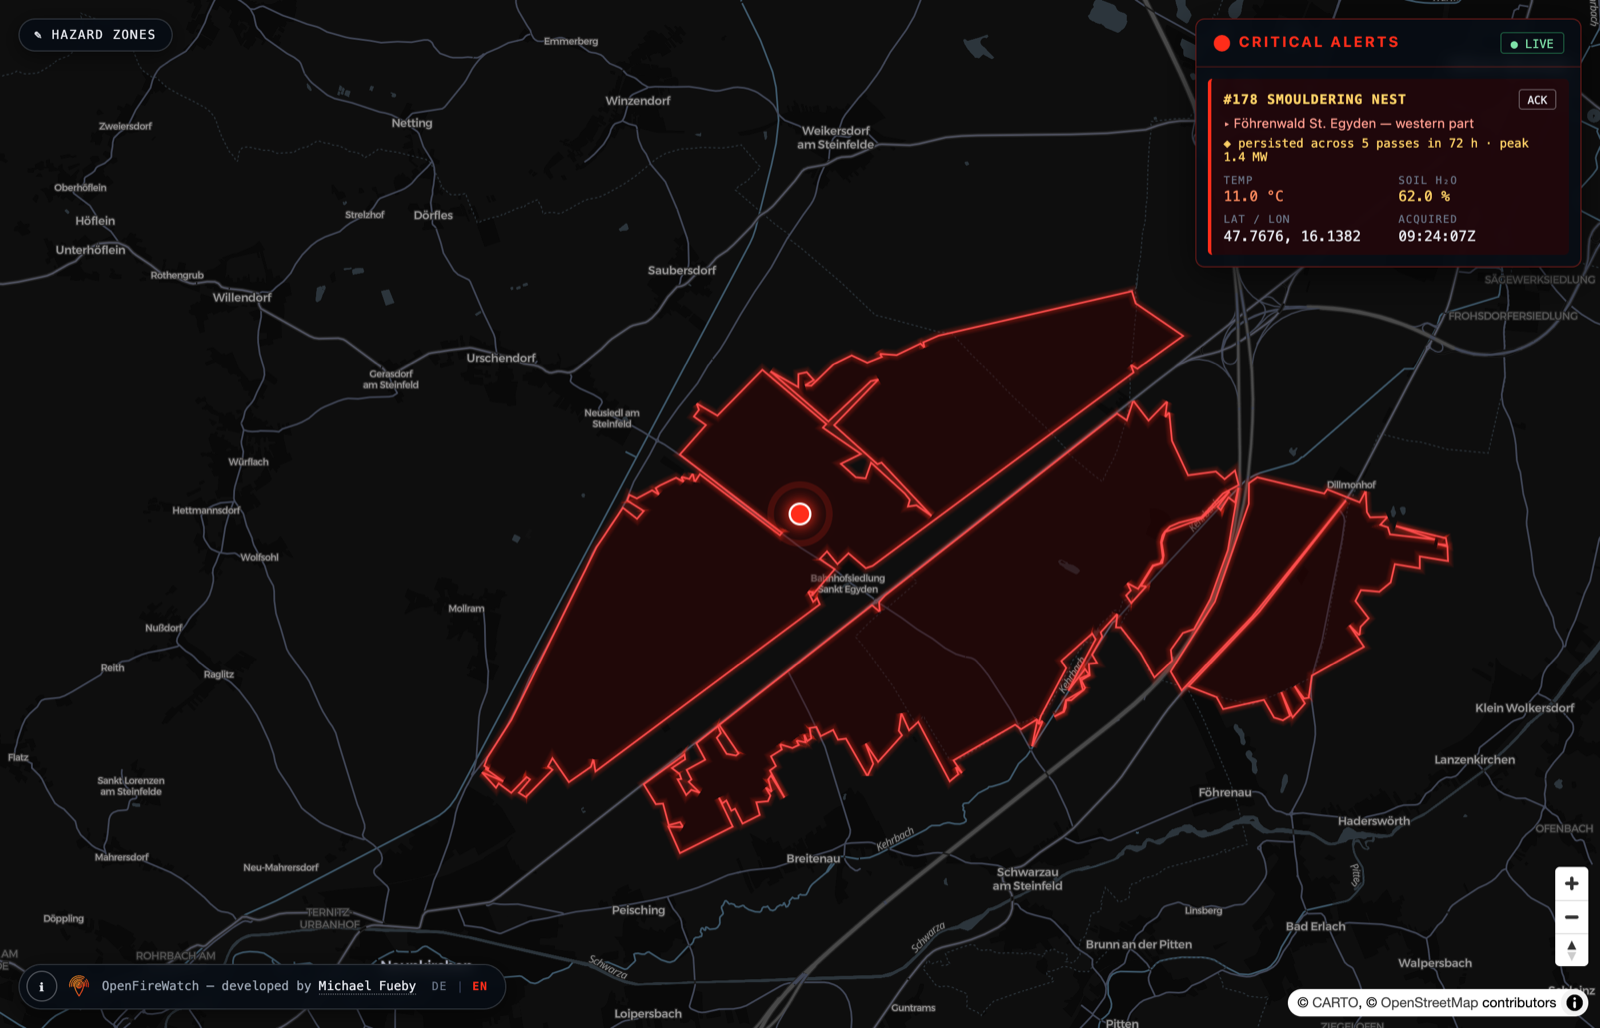
\includegraphics[width=\textwidth]{img/lagekarte.png}

\vfill
{\color{ofwGrau}
Live-Instanz: \url{https://openfirewatch.org}\\
Quellcode: \url{https://github.com/michifueby/OpenFireWatch}\\[0.4cm]
Entwickelt von Michael Fueby \quad$\cdot$\quad Open Source (MIT-Lizenz)\par}
\vspace{1cm}
\end{titlepage}

% =============================================================================
\tableofcontents
\newpage

% =============================================================================
\section{Wie Sie dieses Handbuch lesen}

Dieses Handbuch richtet sich an drei sehr unterschiedliche Lesergruppen. Damit
niemand Kapitel lesen muss, die ihn nicht betreffen, ist jeder Abschnitt
gekennzeichnet.

\begin{center}
\begin{tabularx}{\textwidth}{@{}lX@{}}
\toprule
\textbf{Sie sind\ldots} & \textbf{Dann lesen Sie} \\
\midrule
bei der Feuerwehr oder im Einsatzdienst &
Kapitel \ref{sec:was}, \ref{sec:karte} und \ref{sec:grenzen}. Sie erfahren,
was eine Meldung bedeutet, wie zuverlässig sie ist --- und wo die Grenzen
liegen. \\[4pt]
privat interessiert &
Kapitel \ref{sec:was} und \ref{sec:urteil}. Dort steht in Alltagssprache,
was das System tut und warum. \\[4pt]
Betreiber der Anlage &
zusätzlich Kapitel \ref{sec:zonen}: Gefahrenzonen anlegen, ändern und
stilllegen. \\[4pt]
Entwicklerin oder Entwickler &
zusätzlich Kapitel \ref{sec:technik} und die Verweise am Ende. \\
\bottomrule
\end{tabularx}
\end{center}

\begin{warnung}[Dies ersetzt keinen Notruf]
OpenFireWatch ist ein \emph{ergänzendes} Hilfsmittel. Wer Rauch oder Feuer
sieht, wählt \textbf{122} (Feuerwehr) beziehungsweise \textbf{112} --- sofort
und unabhängig davon, ob dieses System etwas anzeigt. Ein Mensch vor Ort meldet
einen Brand um Stunden schneller als jeder Satellit.
\end{warnung}

% =============================================================================
\section{Was OpenFireWatch tut}\label{sec:was}
\zielgruppe{alle}

OpenFireWatch beobachtet festgelegte Gebiete auf ungewöhnliche Hitze und meldet
Auffälligkeiten auf einer Lagekarte im Internet --- ohne dass jemand etwas
installieren muss.

Der Anlass war regional. Im \textbf{Föhrenwald} im Steinfeld südwestlich von
Wiener Neustadt liegt Phosphormunition aus dem Zweiten Weltkrieg im Boden.
Weißer Phosphor hat eine gefährliche Eigenschaft: Er entzündet sich bei
ungefähr \textbf{30\,\textdegree C von selbst}, sobald er mit Luft in Berührung
kommt. Normalerweise schirmt feuchter Boden ihn ab. Trocknet der Boden nach
längerer Dürre aus, reißt er auf --- und Sauerstoff gelangt an die Munition.
Inzwischen wird auch der Wald bei \textbf{St.\,Egyden am Steinfeld} überwacht,
wo es tatsächlich gebrannt hat.

\subsection*{Die Kette in vier Schritten}

\begin{enumerate}[leftmargin=*]
  \item \textbf{Satellitendaten.} Alle fünf Minuten fragt das System die
    NASA-Satelliten ab. Deren Instrumente messen die Wärmestrahlung der
    Erdoberfläche und melden Punkte, an denen es auffällig heiß ist.
  \item \textbf{Wetterdaten.} Dazu kommen die aktuelle Lufttemperatur und
    Luftfeuchte einer Messstation der GeoSphere Austria sowie die Feuchte der
    obersten Bodenschicht.
  \item \textbf{Bewertung.} Jeder Hitzepunkt wird geprüft: Liegt er in einer
    hinterlegten Gefahrenzone? Und erfüllt er die Kriterien, die für
    \emph{diese Art} von Gefahr gelten?
  \item \textbf{Meldung.} Trifft beides zu, erscheint der Alarm binnen Sekunden
    auf der Karte --- mit Messwerten und exakten Koordinaten.
\end{enumerate}

\begin{hinweis}[Warum nicht einfach „heiß = Alarm"?]
Weil das entweder ständig fehlalarmieren oder echte Gefahren übersehen würde.
Ein Feld in der Sonne ist heiß, ein Fabrikschornstein auch. Umgekehrt ist ein
Waldbrand an einem kühlen Tag trotzdem ein Waldbrand. Deshalb prüft das System
immer \emph{zwei} Dinge: den Ort (liegt es in einer Gefahrenzone?) und die
Umstände, die zu genau dieser Gefahr passen.
\end{hinweis}

% =============================================================================
\section{Die Lagekarte lesen}\label{sec:karte}
\zielgruppe{Einsatzkräfte und alle, die die Karte im Betrieb nutzen}

Die Karte erreichen Sie unter \url{https://openfirewatch.org}. Sie funktioniert
im Browser auf Handy, Tablet und Rechner; es ist keine Anmeldung nötig. Die
Sprache richtet sich nach Ihrem Gerät, unten links können Sie zwischen Deutsch
und Englisch umschalten.

\subsection{Was Sie auf der Karte sehen}

\begin{center}
\begin{tabularx}{\textwidth}{@{}lX@{}}
\toprule
\textbf{Darstellung} & \textbf{Bedeutung} \\
\midrule
Rot umrandete Fläche & Eine \textbf{Gefahrenzone}. Nur innerhalb dieser
Flächen löst eine Detektion einen Alarm aus. \\[4pt]
Kleiner gelber Punkt & Eine erfasste Hitzequelle, die \emph{keinen} Alarm
ausgelöst hat --- zur Einordnung der Lage. \\[4pt]
Pulsierender roter Punkt & Ein \textbf{kritischer Alarm}. Anklicken zeigt alle
Messwerte. \\
\bottomrule
\end{tabularx}
\end{center}

\subsection{Das Lagepanel rechts oben}

\begin{center}
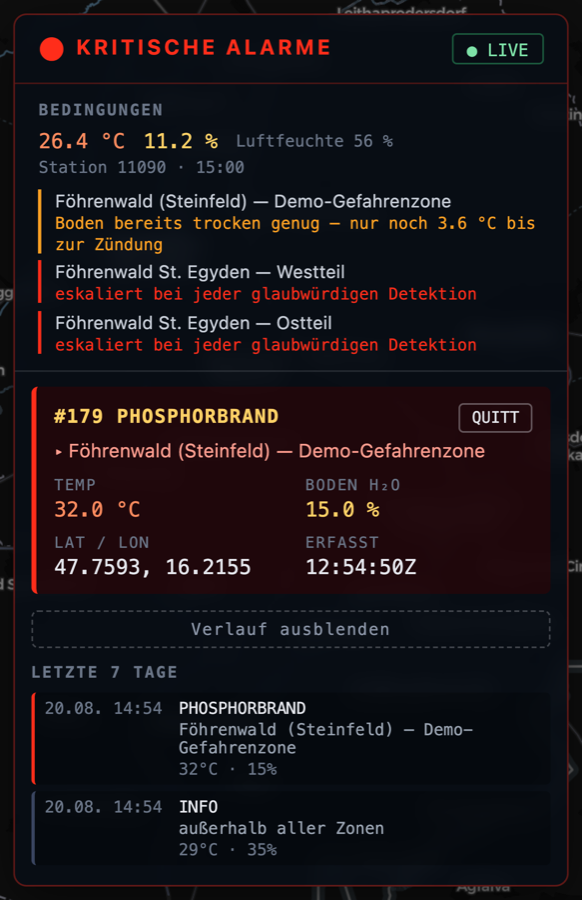
\includegraphics[width=0.62\textwidth]{img/lagepanel.png}
\end{center}

Das Panel hat drei Bereiche, von oben nach unten:

\paragraph{Bedingungen.} Die aktuell gemessenen Werte --- Lufttemperatur,
Bodenfeuchte, Luftfeuchte --- und darunter für jede Zone, \emph{wie weit sie
von einem Alarm entfernt ist}. Das ist der vorausschauende Teil: Sie sehen
morgens, ob heute ein kritischer Tag wird.

Im abgebildeten Beispiel steht beim Föhrenwald \enquote{Boden bereits trocken
genug --- nur noch 3{,}6\,\textdegree C bis zur Zündung}. Das heißt: Eine der
beiden Voraussetzungen für eine Selbstentzündung ist bereits erfüllt, es fehlt
nur noch Wärme. Solche Zonen sind orange markiert.

\paragraph{Aktuelle Alarme.} Jeder Eintrag nennt die Alarmstufe, die betroffene
Zone, Temperatur, Bodenfeuchte, die Koordinaten und den Zeitpunkt der
Satellitenaufnahme. Mit \textbf{QUITT} bestätigen Sie einen Alarm; er
verschwindet dann aus der Liste, bleibt aber im Verlauf erhalten.

\paragraph{Verlauf.} Über \enquote{Verlauf anzeigen} sehen Sie alle Bewertungen
der letzten sieben Tage --- auch die, die zu keinem Alarm geführt haben. Dieser
Bereich beantwortet Fragen wie \enquote{Was war heute Nacht?}.

\subsection{Die Alarmstufen}

\begin{center}
\begin{tabularx}{\textwidth}{@{}l l X@{}}
\toprule
\textbf{Stufe} & \textbf{Farbe} & \textbf{Bedeutung} \\
\midrule
\textsc{Phosphorbrand} & rot &
In einer Phosphor-Zone ist es über 30\,\textdegree C \emph{und} der Boden ist
sehr trocken. Selbstentzündung ist möglich. \\[4pt]
\textsc{Waldbrand} & rot &
In einer Waldbrand-Zone wurde eine glaubwürdige Hitzequelle erfasst. \\[4pt]
\textsc{Hitze an Munitions\-standort} & rot &
Hitze an einem Ort mit Munition --- unabhängig vom Wetter. \\[4pt]
\textsc{Glutnest} & rot &
Eine schwache Wärmequelle blieb über mehrere Satellitenüberflüge am selben
Fleck. Typisches Muster für schwelende Glut. \\[4pt]
\textsc{Thermische Anomalie} & rot &
Auffällige Hitze in einer Zone ohne spezielles Gefahrenmodell. \\[4pt]
\textsc{Erhöht} & orange &
Etwas wurde in einer Zone erfasst, die Kriterien für einen Alarm waren aber
nicht erfüllt. Der Grund wird mit angegeben. \\[4pt]
\textsc{Info} & grau &
Erfasst, aber außerhalb aller Zonen. Erscheint nur im Verlauf. \\
\bottomrule
\end{tabularx}
\end{center}

\begin{hinweis}[Was ein Alarm nicht sagt]
Ein Alarm bedeutet: \emph{Hier ist ungewöhnliche Hitze, und die Umstände passen
zu einer bekannten Gefahr.} Er bedeutet nicht, dass Flammen sichtbar sind, und
er ersetzt keine Erkundung vor Ort. Umgekehrt schließt ein ausbleibender Alarm
ein Feuer nicht aus --- siehe Kapitel \ref{sec:grenzen}.
\end{hinweis}

% =============================================================================
\section{Wie das System zu seinem Urteil kommt}\label{sec:urteil}
\zielgruppe{alle Interessierten}

Entscheidend ist: Für \emph{jede Art} von Gefahr gelten \emph{eigene}
Kriterien. Alles über einen Kamm zu scheren wäre in beide Richtungen falsch.

\begin{center}
\begin{tabularx}{\textwidth}{@{}l X@{}}
\toprule
\textbf{Art der Zone} & \textbf{Wann wird alarmiert} \\
\midrule
Weißer Phosphor &
Nur wenn \textbf{beides} zutrifft: mindestens 30\,\textdegree C \emph{und}
weniger als 20\,\% Bodenfeuchte. Der Mechanismus hängt vom Wetter ab: Bei
feuchtem Boden bleibt die Munition abgeschirmt, bei kühlem Wetter fehlt die
Zündtemperatur. \\[4pt]
Waldbrand &
Bei jeder glaubwürdigen Detektion, \textbf{unabhängig vom Wetter}. Ein
Hitzepunkt im Wald \emph{ist} bereits ein Feuer. Auf 30\,\textdegree C
Lufttemperatur zu warten würde einen echten Brand an einem kühlen Tag
verschweigen. \\[4pt]
Munitionsdepot &
Immer, ohne jede Zusatzbedingung. Hitze an einem Munitionsstandort ist
unabhängig vom Wetter ein Notfall. Ein Fehlalarm ist dort deutlich billiger
als ein übersehener Vorfall. \\[4pt]
Allgemein &
Bei jeder glaubwürdigen Detektion. Auffangfall für Zonen ohne spezielles
Gefahrenmodell. \\
\bottomrule
\end{tabularx}
\end{center}

\subsection*{Glaubwürdigkeit}

Die Satelliten liefern zu jeder Detektion eine eigene Bewertung, wie sicher sie
sich sind. Nur eine ausdrücklich \emph{niedrige} Einstufung unterdrückt einen
Alarm --- so fallen bekannte Störquellen wie Sonnenreflexionen heraus, ohne
dass eine fehlende Angabe stillschweigend zu einer Abwertung führt.

\subsection*{Glutnester}

Eine Flammenfront wandert. Ein Glutnest bleibt liegen und strahlt schwach
weiter. Genau das nutzt das System: Findet es über mindestens zwei getrennte
Satellitenüberflüge hinweg schwache Wärmesignale am selben Fleck (innerhalb von
500\,m und 72 Stunden), meldet es ein mögliches Glutnest. Der Alarm nennt die
Begründung mit, etwa \enquote{bei 4 Überflügen in 72\,h, Spitze 1{,}4\,MW}.

Diese Regel hat Vorrang vor allen anderen: Die Wetterkriterien \emph{sagen
voraus}, dass eine Entzündung wahrscheinlich ist --- eine Persistenz
\emph{beobachtet}, dass bereits etwas brennt.

% =============================================================================
\section{Gefahrenzonen verwalten}\label{sec:zonen}
\zielgruppe{Betreiber der Anlage}

Zonen sind das Einzige, was im laufenden Betrieb gepflegt werden muss. Das
beobachtete Satellitengebiet ergibt sich \emph{automatisch} aus ihnen: Legen
Sie eine Zone an, wird das abgefragte Gebiet beim nächsten Zyklus von selbst
erweitert.

\subsection{Zone anlegen}

\begin{enumerate}[leftmargin=*]
  \item Oben links auf \textbf{Gefahrenzonen} klicken.
  \item \textbf{Entsperren}: den Betreiber-Schlüssel eingeben. Er gilt nur für
    diesen Browser-Tab und ist beim Schließen wieder weg --- das ist Absicht,
    damit an einem gemeinsam genutzten Rechner nichts zurückbleibt.
  \item \textbf{+ Neue Zone} wählen und auf der Karte die Eckpunkte
    anklicken. Die Fläche wird beim Zeichnen angezeigt. Mit
    \enquote{Punkt zurück} nehmen Sie den letzten Punkt zurück, ein Doppelklick
    oder \enquote{Fertig} schließt die Fläche.
  \item Namen auf \textbf{Deutsch und Englisch} eingeben und die Gefahrenart
    wählen. Beide Sprachen sind nötig, weil dieselbe Meldung an Nutzer in
    beiden Sprachen geht.
  \item \textbf{Zone speichern}. Sie erscheint sofort auf der Karte.
\end{enumerate}

\subsection{Zone ändern oder stilllegen}

\textbf{Bearbeiten} ändert Namen und Gefahrenart; über
\enquote{Umriss neu zeichnen} lässt sich die Fläche ersetzen.

\textbf{Stilllegen} beendet die Alarmierung für diese Zone sofort. Sie wird
dabei bewusst \emph{nicht gelöscht}: Alle Alarme, die sie je ausgelöst hat,
bleiben nachvollziehbar. Ohne diesen Schutz würde das Entfernen einer Zone die
Nachweiskette vergangener Ereignisse vernichten.

\begin{hinweis}[Die Wahl der Gefahrenart ist keine Beschriftung]
Sie entscheidet, nach welchen Kriterien bewertet und wie der Alarm benannt
wird. Eine Waldfläche als \enquote{Weißer Phosphor} anzulegen führt dazu, dass
ein echter Waldbrand an einem kühlen Tag nur als \enquote{Erhöht} gemeldet
wird.
\end{hinweis}

% =============================================================================
\section{Was das System nicht kann}\label{sec:grenzen}
\zielgruppe{besonders für Einsatzkräfte --- bitte vollständig lesen}

Diese Grenzen sind keine vorübergehenden Mängel, sondern folgen aus der
Technik. Wer sie kennt, kann die Meldungen richtig einordnen.

\begin{description}[leftmargin=0pt, style=nextline]
  \item[Verdeckte Glut bleibt unsichtbar.]
    Glut, die unter der Erdoberfläche, im Wurzelwerk oder unter geschlossenem
    Kronendach schwelt, sehen die Satelliten \textbf{nicht}. Sie ist zu kühl,
    zu klein und abgeschirmt. Dafür braucht es weiterhin Wärmebildtechnik vor
    Ort oder per Drohne. Was das System findet, ist die \emph{Signatur} an der
    Oberfläche.

  \item[Zeitverzug von Stunden.]
    Ein Satellit sieht einen Ort nur bei seinem Überflug, typischerweise wenige
    Male pro Tag. Zwischen Brandausbruch und Meldung können \textbf{Stunden}
    liegen. Für die schnelle Entdeckung bleiben Menschen, Kameras und
    Beobachtungsflüge unersetzlich.

  \item[Grobe Auflösung.]
    Ein Bildpunkt entspricht etwa 375\,m Kantenlänge. Die gemeldete Position
    ist der Mittelpunkt dieses Bereichs, nicht die exakte Brandstelle.

  \item[Wetter gilt für das Gebiet, nicht für den Punkt.]
    Die Messwerte stammen von einer Wetterstation und einem Bodenfeuchte-Wert
    für das gesamte überwachte Gebiet. Bei kleinen, nahe beieinander liegenden
    Zonen ist das zutreffend; über größere Entfernungen wird es ungenau.

  \item[Die Zonengrenzen sind abgeleitet, nicht amtlich.]
    Die mitgelieferten Flächen stammen aus offenen Kartendaten
    (OpenStreetMap), nicht aus behördlichen Gefahrenkarten. Für den
    verbindlichen Einsatz müssen sie durch die Grenzen der zuständigen Stelle
    ersetzt werden.

  \item[Kein zertifiziertes System.]
    OpenFireWatch ist ein quelloffenes Werkzeug ohne Zulassung als
    Warnsystem, ohne zugesicherte Verfügbarkeit und ohne
    Reaktionszeit-Garantie.
\end{description}

\begin{warnung}[Die wichtigste Regel]
Ein \textbf{ausbleibender Alarm ist kein Nachweis}, dass nichts brennt. Das
System kann Gefahren übersehen --- durch Bewölkung, Verzug, Auflösung oder
verdeckte Glut. Es ergänzt bestehende Verfahren, es ersetzt keines davon.
\end{warnung}

% =============================================================================
\section{Technischer Überblick}\label{sec:technik}
\zielgruppe{Entwicklerinnen und Entwickler}

\subsection{Datenquellen}

\begin{center}
\begin{tabularx}{\textwidth}{@{}l l X@{}}
\toprule
\textbf{Quelle} & \textbf{Liefert} & \textbf{Anmerkung} \\
\midrule
NASA FIRMS (VIIRS) & Hitzepunkte & Zugangsschlüssel nötig, kostenfrei;
5000 Abfragen je 10 Minuten, genutzt werden 2 \\
GeoSphere Austria & Temperatur, Luftfeuchte & Station des TAWES-Netzes,
ohne Schlüssel \\
Open-Meteo & Bodenfeuchte & oberste Schicht (1--3\,cm), ohne Schlüssel \\
OpenStreetMap & Zonengeometrie & Grundlage der mitgelieferten Zonen \\
\bottomrule
\end{tabularx}
\end{center}

\subsection{Aufbau}

Fünf Dienste, gestartet mit einem einzigen Befehl über Docker Compose:

\begin{description}[leftmargin=0pt, style=nextline, itemsep=2pt]
  \item[workers] Hintergrundprozesse (Node.js, BullMQ), die die externen
    Schnittstellen abfragen. Fehlversuche werden mit wachsendem Abstand
    wiederholt; endgültig gescheiterte Aufträge landen in einer eigenen
    Warteschlange und gehen nie verloren.
  \item[redis] Nachrichtenbus. Entkoppelt die Dienste, sodass jeder einzeln
    neu starten kann, ohne dass Daten verloren gehen.
  \item[db] PostgreSQL mit PostGIS. Die räumliche Prüfung findet in der
    Datenbank statt (\texttt{ST\_Intersects} auf einem GiST-Index), nicht im
    Anwendungscode.
  \item[backend] NestJS. Bewertet die Meldungen, stellt die REST-Schnittstelle
    samt OpenAPI-Dokumentation bereit und verteilt Alarme über WebSockets.
  \item[frontend] Angular mit MapLibre GL JS, ausgeliefert von nginx.
\end{description}

\subsection{Schnittstelle}

Lesende Zugriffe sind öffentlich, schreibende benötigen den Betreiber-Schlüssel
im Kopffeld \texttt{X-API-Key}. Ist kein Schlüssel konfiguriert, werden
schreibende Zugriffe abgewiesen statt ungeschützt zugelassen.

\begin{center}
\begin{tabularx}{\textwidth}{@{}l l X@{}}
\toprule
\textbf{Methode} & \textbf{Pfad} & \textbf{Zweck} \\
\midrule
GET & \texttt{/api/health} & Betriebsprüfung \\
GET & \texttt{/api/risk-zones} & Zonen als GeoJSON \\
GET & \texttt{/api/anomalies} & erfasste Hitzepunkte \\
GET & \texttt{/api/alerts} & Verlauf der Bewertungen \\
GET & \texttt{/api/conditions} & Bedingungen und Zonenbereitschaft \\
POST & \texttt{/api/risk-zones} & Zone anlegen \quad\textbf{(Schlüssel)} \\
PUT & \texttt{/api/risk-zones/\{id\}} & Zone ersetzen \quad\textbf{(Schlüssel)} \\
DELETE & \texttt{/api/risk-zones/\{id\}} & Zone stilllegen \quad\textbf{(Schlüssel)} \\
POST & \texttt{/api/simulate-fire} & Probealarm \quad\textbf{(Schlüssel)} \\
\bottomrule
\end{tabularx}
\end{center}

Die vollständige, stets aktuelle Beschreibung steht unter
\url{https://openfirewatch.org/api/docs}.

\subsection{Selbst betreiben}

\begin{verbatim}
git clone https://github.com/michifueby/OpenFireWatch.git
cd OpenFireWatch
cp .env.example .env      # FIRMS-Schlüssel und Passwörter eintragen
docker compose up --build
\end{verbatim}

Danach ist die Karte unter \texttt{http://localhost:4200} erreichbar. Der
öffentliche Betrieb mit TLS ist in \texttt{docs/deployment.md} beschrieben.

\subsection{Mitarbeiten}

Rückmeldungen sind ausdrücklich erwünscht --- besonders aus der Einsatzpraxis.
Die fachlichen Annahmen (Schwellenwerte, benötigte Angaben im Alarm, sinnvolle
Zonengrenzen) stammen von einem Entwickler, nicht von einer Einsatzkraft.
Kritik daran ist wertvoller als Zustimmung.

\begin{itemize}[leftmargin=*, itemsep=1pt]
  \item Fehler und Vorschläge: \url{https://github.com/michifueby/OpenFireWatch/issues}
  \item Mitwirken: Datei \texttt{CONTRIBUTING.md} im Projekt
  \item Sicherheitslücken: bitte \emph{nicht} öffentlich melden, siehe
    \texttt{SECURITY.md}
\end{itemize}

% =============================================================================
\vfill
\begin{center}
\color{ofwGrau}\small
Kartengrundlage \textcopyright\ CARTO und OpenStreetMap-Mitwirkende \quad$\cdot$\quad
Satellitendaten: NASA FIRMS \quad$\cdot$\quad Wetterdaten: GeoSphere Austria, Open-Meteo\\
OpenFireWatch ist ein unabhängiges Projekt und steht in keiner Verbindung zur NASA.
\end{center}

\end{document}
